\chapter{Introducción a las cadenas de Markov}
En este capítulo vamos a inicializar la teoría de cadenas de Markov, avanzado progresivamente hacia las cadenas de Markov ocultas. En primer lugar, vamos a presentar el concepto de procesos de Markov:

\section{Propiedad de Markov}
Sea $\mathbb{S}$ un conjunto finito de forma $\{s_1,...,s_n\}$, definimos un proceso estocástico sobre $\mathbb{S}$ como una secuencia de variables aleatorias $\{\mathcal{X}_0,\mathcal{X}_1,\mathcal{X}_2,...\}$, o $\{\mathcal{X}_t\}_{t=0}^{\infty}$ para acortar, donde cada $\mathcal{X}_t$ es una variable aleatoria que toma valores en $\mathbb{S}$.


 A pesar de que el índice $t$ puede representar cualquiera magnitud, lo más común es que represente el tiempo. Si tomamos el índice $t$ como el tiempo, obtenemos la noción de \enquote{pasado} y \enquote{futuro}, esto es, si $t<t'$, entonces $\mathcal{X}_t$ es una variable \enquote{pasada} para $\mathcal{X}_{t'}$, mientras que $\mathcal{X}_{t'}$ es una variable \enquote{futura} para $\mathcal{X}_t$. Sin embargo, esto no es siempre así, por ejemplo, si el proceso estocástico corresponde al de las secuencias de genomas de un organismo, el conjunto $\mathbb{S}$ estará formado por los cuatro símbolos para las subunidades de nucleótidos $\{A,C,G,T\}$ y las secuenciaciones tienen un significado más espacial que temporal.
 
\begin{definition}
Un proceso estocástico $\{\mathcal{X}_t\}_{t=0}^{\infty}$ se dice que posee \textbf{la propiedad de Markov}, o es un \textbf{proceso de Markov}, si para todo $t\geq1$ y $(u_0,...,u_{t-1},u_t)\in\mathbb{S}^{t+1}$ se tiene que:
\[ \tag{1.\arabic{CadeanasMarkov}}\label{eqDefMarkov}
    P[\mathcal{X}_t=u_t|\mathcal{X}_0=u_0,...,\mathcal{X}_{t-1}=u_{t-1}]=P[\mathcal{X}_t=u_t|\mathcal{X}_{t-1}=u_{t-1}]
\]
\end{definition}

La propiedad de Markov afirma que las distribuciones condicionadas del \enquote{estado actual} $\mathcal{X}_t$ depende únicamente del \enquote{pasado inmediato} $\mathcal{X}_{t-1}$ y no depende de ninguno de los anteriores estados. 

Por conveniencia, introducimos la notación $\mathcal{X}_j^k$ para denotar los estados $\mathcal{X}_i$ con $j\leq i\leq k$. Con esta notación, podemos reescribir la Definición 1.1 como sigue: Un proceso estocástico $\{\mathcal{X}_t\}$ es un \textbf{proceso de Markov} si, para todo $(u_0,...,u_{t-1},u_t)\in\mathbb{S}^{t+1}$ es cierto que:
\[  \stepcounter{CadeanasMarkov}
    \tag{1.\arabic{CadeanasMarkov}}\label{eqDefMarkov2}
    P[\mathcal{X}_t=u_t|\mathcal{X}_0^{t-1}=u_0...u_{t-1}]=P[\mathcal{X}_t=u_t|\mathcal{X}_{t-1}=u_{t-1}]
\]

Para cualquier proceso estocástico $\{\mathcal{X}_t\}$ y cualquiera secuencia $(u_0,...,u_{t-1},u_t)\in\mathbb{S}^{t+1}$, tenemos que por definición de probabilidad condicionada:

\[
P[\mathcal{X}_0^t=u_0...u_t]=P[\mathcal{X}_0=u_0]\cdot\prod_{i=0}^{t-1}P[\mathcal{X}_{i+1}=u_{i+1}|\mathcal{X}_0^i=u_0...u_i]
\]

Sin embargo, si consideramos un proceso de Markov, entonces la fórmula anterior se reduce a:
\[ \stepcounter{CadeanasMarkov}
\tag{1.\arabic{CadeanasMarkov}} \label{propiedadMarkov}
P[\mathcal{X}_0^t=u_0...u_t]=P[\mathcal{X}_0=u_0]\cdot\prod_{i=0}^{t-1}P[\mathcal{X}_{i+1}=u_{i+1}|\mathcal{X}_i=u_i]
\]

En probabilidad, es usual referirse con el nombre \textbf{cadena de Markov} a un proceso de Markov $\mathcal{X}_t$ donde el parámetro $t$ toma únicamente valores discretos. En este trabajo, pondremos nuestra atención en los casos donde $t$ toma valores en $\mathbb{N}_0$.

En (\ref{propiedadMarkov}) vemos la importancia del valor:
\[
P[\mathcal{X}_{t+1}=u|\mathcal{X}_t=v]
\]

al que podemos identificar como una función de tres variables: el estado \enquote{actual} $v\in\mathbb{S}$, el estado \enquote{siguiente} $u\in\mathbb{S}$ y el \enquote{tiempo actual} $t\in\mathbb{N}_0$. Así, teniendo en cuenta que $\mathbb{S}=\{s_1,...,s_n\}$ definimos para todo tiempo $t\in\mathbb{N}_0$ la probabilidad de transición:

\[ \stepcounter{CadeanasMarkov}
\tag{1.\arabic{CadeanasMarkov}} \label{compTransición}
a_{ij}(t):=P[\mathcal{X}_{t+1}=s_j|\mathcal{X}_t=s_i]
\]

Por tanto, $a_{ij}(t)$ es la probabilidad de realizar una transición desde el estado actual $s_i$ al estado siguiente $s_j$ en el instante $t$.

\begin{definition}
Sea $\mathcal{X}_t$ una cadena de Markov, la matriz cuadrada de dimensión $n$,  $A(t)=[a_{ij}(t)]$, es la \textbf{matriz de transición} de $\mathcal{X}_t$ en el instante $t$. Una cadena de Markov es \textbf{homogénea} si $A(t)$ es constante para todo $t\in\mathbb{N}_0$, en otro caso, es \textbf{no homogénea}. 
\end{definition}

\begin{definition}
Sea $\mathcal{X}_t$ una cadena de Markov tomando valores en un conjunto finito $\mathbb{S}=\{s_1,...,s_n\}$, y sea $A(t)$ su matriz de transición en el instante $t$. Entonces, $A(t)$ es una \textbf{matriz estocástica} (por filas) para todo $t$, esto es:
\begin{align*}
a_{ij}(t)\in[0,1],\, \forall i,j \in \{1,...,n\}, t\in\mathbb{N}_0\\
\sum_{j=1}^n a_{ij}(t)=1, \, \forall i\in\{1,...,n\}, t\in\mathbb{N}_0
\end{align*}
\end{definition}

\begin{lemma}
Sea $A$ una matriz positiva de dimensión $n\times n$:
\begin{enumerate}
    \item $A$ es estocástica si y solo si 1 es un valor propio de $A^T$ con vector propio (a la izquierda) $\bold{1}=\begin{pmatrix}1 & 1 & \dots & 1\end{pmatrix}$.
    \item si $A$ es estocástica, entonces para todo valor propio $\lambda$, se cumple que  $\left|\lambda\right|\leq1.$
\end{enumerate}
\end{lemma}

\begin{proofs*}
\
\begin{enumerate}
    \item Es suficiente con observar que la condición de estocaticidad para una matriz positiva $A$ es equivalente a que $\bold{1}\cdot A^T=\bold{1}$.
    \item Sea $v$ un vector propio asociado (a izquierda pues estamos usando la notación fila) a $\lambda$, por ser $A$ positiva y estocástica, tenemos que:
    \[
    \left|\lambda\right|\sum_{j=1}^n\left| v_j\right|=\sum_{j=1}^n\left|\lambda v_j\right|= \sum_{j=1}^n\left|(vA)_j \right|  =\sum_{j=1}^n\left|\sum_{i=1}^n a_{ij}v_i\right|\]
    \[\leq\sum_{j=1}^n\sum_{i=1}^n a_{ij}\left|v_i\right|=\sum_{i=1}^n\left( \sum_{j=1}^n a_{ij} \right) \left|v_i\right|=\sum_{i=1}^n\left|v_i\right|\]
    Puesto que $\sum_{r=1}^n\left|v_r\right|\neq0$, tenemos que $\left|\lambda\right|\leq1$.\qed
\end{enumerate}
\end{proofs*}
Para continuar con los estudios de las cadenas de Markov presentamos el siguiente conjunto:

\begin{definition}
El \textbf{n-símplex estándar} es el subconjunto de $\mathbb{R}^{n+1}$ dado por:
\[
\Delta^n=\{(t_1,...,t_{n+1})\in \mathbb{R}^{n+1} \, |\, \sum_{i=1}^{n+1} t_i=1 \text{ y } t_i\geq0 \text{ para todo } i\}
\]
\end{definition}

\begin{lemma}
Sea $\{\mathcal{X}_t\}$ una cadena de Markov con valores en $\mathbb{S}=\{s_1,...,s_n\}$, y sea $A(t)$ su matriz de transición en el instante $t$. Supongamos que el estado inicial $\mathcal{X}_0$ se distribuye de acuerdo con $c^0 \in \Delta^{n-1}$, esto es:
\[
P[\mathcal{X}_0=s_i]=c_i^0,\, \forall i \in \{1,...,n\}
\]
Entonces, para todo $t\geq0$, el estado $\mathcal{X}_t$ se distribuye de acuerdo con:
\[\stepcounter{CadeanasMarkov}
\tag{1.\arabic{CadeanasMarkov}} \label{fórmulaDistribuciónEnT}
c^t=c^0A(0)A(1)\cdot\cdot\cdot A(t-1)
\]
\end{lemma}

\begin{proofs*}
Sea $s_i\in \mathbb{S}$, por \ref{propiedadMarkov} tenemos que:

\[P[\mathcal{X}_t=s_i]=\]
\[\sum_{u_0u_1...u_{t-1}\in\mathbb{S}^{t}}P[\mathcal{X}_0=u_0]\cdot\prod_{i=0}^{t-2}P[\mathcal{X}_{i+1}=u_{i+1}|\mathcal{X}_i=u_i]\cdot P[\mathcal{X}_t=s_i|\mathcal{X}_{t-1}=u_{t-1}] \]
\[=\sum_{u_0u_1...u_{t-1}\in\mathbb{S}^{t}}c_{u_0}\cdot a_{u_0,u_1}(0)\cdot\cdot\cdot a_{u_{t-2},u_{t-1}}(t-2)\cdot a_{u_{t-1},s_i}(t-1)\]
Notemos que esta última expresión es justamente la componente $i$-ésima de $c^t=c^0A(0)A(1)\cdot\cdot\cdot A(t-1)$ escrita en forma extensa.\qed
\end{proofs*}

\begin{exampleth}
En este ejemplo presentamos una variación del juego de cartas \enquote{blackjack}. En este caso, tenemos un dado de cuatro caras con valores 0, 1, 2 y 3, y con probabilidad uniforme en cada lanzamiento. Un jugador lanza el dado de forma repetida y $\mathcal{X}_t$ representa el valor acumulado tras $t$ lanzamientos. Si el total es igual a nueve, el jugador gana; en otro caso se considera que pierde. Podemos asumir que el resultado de cada lanzamiento es independiente de los lanzamientos anteriores.

Tenemos entonces que $\{\mathcal{X}_t\}$ toma valores en el conjunto $\mathbb{S}:=\{0,1,...,8,W,L\}$ de cardinalidad 11. Sea $\mathcal{Y}_t$ el resultado del lanzamiento en el instante $t$:
\[
P[\mathcal{Y}_t=0]=P[\mathcal{Y}_t=1]=P[\mathcal{Y}_t=2]=P[\mathcal{Y}_t=3]=1/4
\]

Examinemos ahora la distribución de $\mathcal{X}_t$, por definición sabemos que $\mathcal{X}_t=\mathcal{X}_{t-1}+\mathcal{Y}_t$, excepto el caso de que $\mathcal{X}_{t-1}+\mathcal{Y}_t=9$, consideraremos $\mathcal{X}_t=W$ (ganar); y si $\mathcal{X}_{t-1}+\mathcal{Y}_t>9$, consideraremos $\mathcal{X}_t=L$ (perder). Si $\mathcal{X}_{t-1}=W$ o $L$, consideraremos que el juego está acabado y $\mathcal{X}_t=\mathcal{X}_{t-1}$. Estas observaciones se pueden resumir en las siguientes reglas:

\begin{itemize}
    \item Si $\mathcal{X}_{t-1}\leq5$:
    \[
    P[\mathcal{X}_t=\mathcal{X}_{t-1}]=P[\mathcal{X}_t=\mathcal{X}_{t-1}+1]=\]\[=P[\mathcal{X}_t=\mathcal{X}_{t-1}+2]=P[\mathcal{X}_t=\mathcal{X}_{t-1}+3]=1/4
    \]
    \item Si $\mathcal{X}_{t-1}=6$:
    \[
    P[\mathcal{X}_t=6]=P[\mathcal{X}_t=7]=P[\mathcal{X}_t=8]=P[\mathcal{X}_t=W]=1/4
    \]
    \item Si $\mathcal{X}_{t-1}=7$:
    \[
    P[\mathcal{X}_t=7]=P[\mathcal{X}_t=8]=P[\mathcal{X}_t=W]=P[\mathcal{X}_t=L]=1/4
    \]
    \item Si $\mathcal{X}_{t-1}=8$:
    \[
        P[\mathcal{X}_t=8]=P[\mathcal{X}_t=W]=1/4
    \]\[
        P[\mathcal{X}_t=L]=1/2
    \]
    \item Si $\mathcal{X}_{t-1}=W$ o $L$:
    \[
        P[\mathcal{X}_t=\mathcal{X}_{t-1}]=1
    \]
\end{itemize}

$\{\mathcal{X}_t\}$ es una cadena de Markov pues la distribución de $\mathcal{X}_t$ depende únicamente del valor de $\mathcal{X}_{t-1}$ y no de cómo se ha alcanzado dicho valor. Notemos que las probabilidades anteriores no dependen de $t$, con lo cual la matriz de transición de $\mathcal{X}_t$ es una matriz fija y $\mathcal{X}_t$ es homogénea. 

La matriz de transición de $\mathcal{X}_t$ es entonces una matriz 11$\times$11 dado por:

\begin{center}
    $A=\begin{pmatrix}
    1/4 & 1/4 & 1/4 & 1/4 & 0 & 0 & 0 & 0 & 0 & 0 & 0 \\   
    0 & 1/4 & 1/4 & 1/4 & 1/4 & 0 & 0 & 0 & 0 & 0 & 0 \\
    0 & 0 & 1/4 & 1/4 & 1/4 & 1/4 & 0 & 0 & 0 & 0 & 0 \\
    0 & 0 & 0 & 1/4 & 1/4 & 1/4 & 1/4 & 0 & 0 & 0 & 0 \\
    0 & 0 & 0 & 0 & 1/4 & 1/4 & 1/4 & 1/4 & 0 & 0 & 0 \\
    0 & 0 & 0 & 0 & 0 & 1/4 & 1/4 & 1/4 & 1/4 & 0 & 0 \\
    0 & 0 & 0 & 0 & 0 & 0 & 1/4 & 1/4 & 1/4 & 1/4 & 0 \\
    0 & 0 & 0 & 0 & 0 & 0 & 0 & 1/4 & 1/4 & 1/4 & 1/4 \\
    0 & 0 & 0 & 0 & 0 & 0 & 0 & 0 & 1/4 & 1/4 & 2/4 \\
    0 & 0 & 0 & 0 & 0 & 0 & 0 & 0 & 0 & 1 & 0 \\
    0 & 0 & 0 & 0 & 0 & 0 & 0 & 0 & 0 & 0 & 1 \\
    \end{pmatrix}$
\end{center}

Es natural que el juego comience con el valor inicial igual a cero. Por lo tanto, la distribución de $\mathcal{X}_0$ está representada por $c_0\in\mathbb{R}^{11}$ con un 1 en la primera componente y ceros en el resto. Aplicando repetidamente la fórmula \ref{fórmulaDistribuciónEnT} obtendremos las distribuciones de $\mathcal{X}_1,\,\mathcal{X}_2,$ etc. Así, sea $c_t$ la distribución de $\mathcal{X}_t$, tenemos:
\[
c_0=\begin{pmatrix}
1 & 0 & \dots & 0
\end{pmatrix}\]
\[
c_1=c_0A=\begin{pmatrix}
1/4 & 1/4 & 1/4 & 1/4 & 0 & \dots & 0
\end{pmatrix}\]
\[
c_2=c_1A=\begin{pmatrix}
1/16 & 1/8 & 3/16 & 1/4 & 3/16 & 1/8 & 1/16  & 0 & 0 & 0 & 0
\end{pmatrix}
\]

Cabe destacar que si examinamos la distribución $c_t$, entonces tenemos que $P[\mathcal{X}_t\in\{0\dots8\}]$ tiende a cero conforme $t\rightarrow\infty$. Esto es natural pues el juego terminará eventualmente en victoria ($W$) o en pérdida ($L$) y todos los otros estados son transitorias. Esta idea, nos introduce al siguiente apartado.

\end{exampleth}

\section{Estados de una cadena de Markov}
A partir de esta sección, vamos a centrarnos en el estudio de cadenas de Markov cuyas matrices de transición son constantes, en consecuencia, las probabilidades de transición son independientes del instante $t$. Nos referiremos a ellas directamente como cadenas de Markov, asumiendo homogeneidad. \\

Está claro que los estados juegan un papel importante en el estudio de las cadenas de Markov, para describir con más detalles las propiedades de una cadena de Markov vamos a distinguir los estados que puede tener. Antes de empezar la clasificación, nos interesa saber cómo evoluciona una cadena de Markov tras $n$ instantes:


\begin{definition}
Sea $\{\mathcal{X}_t\}$ una cadena de Markov, $s_i, s_j \in \mathbb{S}$, $n,m\in\mathbb{N}_0$, denotamos:
\[P_{ij}^{m,m+n}:=P[\mathcal{X}_{n+m}=s_j|\mathcal{X}_m=s_i]\]
Si $n=0$:
\[P_{ij}^{m,m}=P[\mathcal{X}_{m}=s_j|\mathcal{X}_m=s_i]=\delta_{ij}=
\begin{cases}
    1, & \text{si } i=j\\
    0, &         \text{si } i\neq j
\end{cases}\]
\end{definition}
\begin{theorem}[Ecuación de Chapman-Kolmogorov]
En condiciones anteriores, sea $r\in \mathbb{N}_0$:
\[P_{ij}^{m,m+n+r}=\sum_{s_k\in\mathbb{S}}P_{ik}^{m,m+n}P_{kj}^{m+n,m+n+r}\]
\end{theorem}
\begin{proofs*}
    \[ P_{ij}^{m,m+n+r}=P[\mathcal{X}_{m+n+r}=s_j|\mathcal{X}_m=s_i]\]
    \[=\sum_{s_k\in\mathbb{S}} P[\mathcal{X}_{m+n+r}=s_j |\mathcal{X}_{m+n}=s_k,\mathcal{X}_m=s_i ] P[\mathcal{X}_{m+n}=s_k|\mathcal{X}_m=s_i ]\]
Aplicando la propiedad de Markov:
    \[P[\mathcal{X}_{m+n+r}=s_j |\mathcal{X}_{m+n}=s_k,\mathcal{X}_m=s_i ]\]\[=P[\mathcal{X}_{m+n+r}=s_j |\mathcal{X}_{m+n}=s_k]=P_{kj}^{m+n,m+n+r}\]
Por lo tanto:
    \[
    \pushQED{\qed}
    P_{ij}^{m,m+n+r}=\sum_{s_k\in\mathbb{S}}P_{ik}^{m,m+n}P_{kj}^{m+n,m+n+r}\qedhere
    \popQED\]
    
\end{proofs*}

Notemos que por ser $\{\mathcal{X}_t\}$, $P_{ij}^{m,m+1}$ es independiente de $m$, por lo cual aplicando inductivamente la ecuación de Chapman-Kolmogorov, tenemos que $P_{ij}^{m,m+n}$ son independientes de $m$. 
\begin{definition}
Sea $\{\mathcal{X}_t\}$ una cadena de Markov, $s_i, s_j \in \mathbb{S}$, $n,m\in\mathbb{N}_0$,  definimos las probabilidades de transición en $n$ pasos como:
\[a_{ij}^{(n)}:=P_{ij}^{m,m+n}=P[\mathcal{X}_{m+n}=s_j|\mathcal{X}_m=s_i]\]
Y la matriz de las probabilidades de transición en $n$ pasos como $A^{(n)}=[a_{ij}^{(n)}]$.
\end{definition}
\begin{lemma}
La matriz de transición en $n$ pasos cumple que $A^{(n)}=A^n, \forall n\in\mathbb{N}$.
\end{lemma}
\begin{proofs*}
 Expresando la ecuación de Chapman-Kolmogorov en forma matricial tenemos que $A^{(n+r)}=A^{(n)}A^{(r)}$, por ser $A^{(1)}=A$:
    \[
    \pushQED{\qed}
    A^{(n)}=A^{(n-1)}A=A^{(n-2)}A^2=\dots=A^n \qedhere
    \popQED\]    
\end{proofs*}

\subsection{Estados alcanzables y comunicables}
\begin{definition}
    El estado $s_j$ se dice \textbf{alcanzable} o \textbf{accesible} desde el estado $s_i$, representado por $i\longrightarrow j$, si existe $n\in\mathbb{N}_0$ tal que $a_{ij}^{(n)}>0$. \\
    Dos estados, $s_i$ y $s_j$, que son mutuamente alcanzables, se dicen \textbf{comunicables}, representado por $i\longleftrightarrow j$.
\end{definition}

La definición anterior tiene el significado siguiente: si $s_j$ es accesible desde el estado $s_i$, entonces existirá un $n\in\mathbb{N}_0$ tal que $P[\mathcal{X}_{m+n}=s_j]>0$ siempre que $\mathcal{X}_m=s_i$.  Es decir, empezando desde el estado $s_i$, hay una probabilidad positiva de que, en un número finito de transiciones, alcancemos el estado $s_j$.

\begin{theorem}
    La propiedad de comunicación, $\longleftrightarrow$, es una relación de equivalencia sobre el conjunto de estados $\mathbb{S}$.
\end{theorem}
\begin{proofs*}
    \
    \begin{itemize}
        \item $\textbf{Reflexividad: } a_{ii}^{(0)}=\delta_{ii}=1>0$. Por tanto, $i\longleftrightarrow i$.
        \item $\textbf{Simetría:}$ si $i\longleftrightarrow j$, existen $n,m\in\mathbb{N}_0$ tales que $a_{ij}^{(n)}, a_{ji}^{(m)}>0$, escogiendo los mismos $n$ y $m$, tenemos que $j\longleftrightarrow i$.
        \item $\textbf{Transitividad:}$ sean $i\longleftrightarrow j$ y $j\longleftrightarrow k$:
        \begin{itemize}
            \item Por ser $i\longleftrightarrow j$, existen $n,m\in\mathbb{N}_0$ tales que $a_{ij}^{(n)}, a_{ji}^{(m)}>0$.
            \item Por ser $j\longleftrightarrow k$, existen $r,s\in\mathbb{N}_0$ tales que $a_{jk}^{(r)}, a_{kj}^{(s)}>0$.
        \end{itemize}
        Aplicando entonces la ecuación de Chapman-Kolmogorov tenemos que:
        \begin{itemize}
            \item $a_{ik}^{(n+r)}=\sum\limits_{s_l\in\mathbb{S}}a_{il}^{(n)}a_{lk}^{(r)}\geq a_{ij}^{(n)}a_{jk}^{(r)}>0$
            \item $a_{ki}^{(s+m)}=\sum\limits_{s_l\in\mathbb{S}}a_{kl}^{(s)}a_{li}^{(m)}\geq a_{kj}^{(s)}a_{ji}^{(m)}>0$
        \end{itemize}
        Por lo tanto, $i\longleftrightarrow k$.\qed
    \end{itemize}
\end{proofs*}

Como resultado, podemos dividir el conjunto de los estados $\mathbb{S}$ en clases de equivalencias dependiendo de si existen comunicaciones entre los estados. Esto introduce a la siguiente definición:
\begin{definition}
    Sea $\{\mathcal{X}_t\}$ una cadena de Markov sobre un conjunto finito $\mathbb{S}$, $\{\mathcal{X}_t\}$ es \textbf{irreducible} si hay solo una clase de equivalencia sobre $\mathbb{S}$ mediante la relación $\longleftrightarrow$.
\end{definition}

Es decir, una cadena de Markov es irreducible si todos los estados se comunican unos con otros. Tomando el ejemplo de \enquote{blackjack}, podemos apreciar que:
    \begin{itemize}
        \item Un estado $s_i\in \{0\dots 8\}$ no es comunicable con un estado $s_j$ con valor inferior $\Longrightarrow a_{ij}^{(n)}=0, \forall n\in\mathbb{N}_0, j<i$.
        \item Los estados $W$ y $L$ no son modificables $\Longrightarrow a_{Wi}^{(n)}=a_{Li}^{(n)}=0, \forall n\in\mathbb{N}_0,  i \in \{0\dots 8, W$ o $L\}$
    \end{itemize}

Por simetría, cada estado es únicamente comunicable consigo mismo. En consecuencia, hay 11 clases de equivalencia en $\mathbb{S}$, uno por cada estado y la cadena de Markov no es irreducible.

\subsection{Periodicidad de una cadena de Markov}
\begin{definition}
Sea $a_{ii}^{(n)}$ la probabilidad de transición en $n$ pasos al estado $s_i$ desde $s_i$, el periodo $\lambda(i)$ de un estado $s_i$ es el máximo común divisor de todos los $n\in\mathbb{N}$ con $a_{ii}^{(n)}>0$, esto es:
\[
\lambda(i):=m.c.d(\{n\in\mathbb{N}\,|\, a_{ii}^{(n)}>0\})
\]
Si $a_{ii}^{(n)}=0$ para todo $n\in\mathbb{N}$, entonces definimos $\lambda(i):=0$.
\end{definition}
A continuación indicamos que la periodicidad también es una propiedad de clase. Esto es, si el estado $s_i$ en una clase tiene periodo $t$, entonces todos los estados de esa clase tienen periodo $t$.
\begin{theorem}
    Si $i\longleftrightarrow j$, entonces $\lambda(i)=\lambda(j)$, es decir, el periodo es constante en cada clase de equivalencia.
\end{theorem}
\begin{proofs*}
Si $i=j$ el resultado es trivial. Supongamos que $i\neq j$, entonces existen $n,m\in\mathbb{N}$ tales que $a_{ij}^{(n)},a_{ji}^{(m)}>0$, por la ecuación de Chapman-Kolmogorov:
\[ a_{ii}^{(n+m)}=\sum\limits_{s_l\in\mathbb{S}}a_{il}^{(n)}a_{li}^{(m)}\geq a_{ij}^{(n)}a_{ji}^{(m)}>0\Longrightarrow\lambda(i)\,|\,(n+m)\]
Sea $s\in\mathbb{N}$ tal que $a_{jj}^{(s)}>0$:
\[ a_{ii}^{(n+m+s)}\geq a_{ij}^{(n)}a_{jj}^{(s)}a_{ji}^{(m)}>0\Longrightarrow \lambda(i)\,|\,(n+m+s)\]
Por lo tanto, $\lambda(i)\,|\,s$, como $s$ es arbitrario, $\lambda(i)$ es un divisor común de $\{n\in\mathbb{N}\,|\, a_{jj}^{(n)}>0\}$, por definición de periodo, $\lambda(i)\,|\,\lambda(j)$. Realizando la misma discusión intercambiando los papeles de $i$ y $j$, obtenemos que $\lambda(j)\,|\,\lambda(i)$, por lo tanto, $\lambda(i)=\lambda(j)$. \qed
\end{proofs*}

\begin{definition}
Un estado $s_i$ se dice \textbf{no periódico} o \textbf{aperiódico} si $\lambda(i)=1$. 
\end{definition}
\begin{definition}
Si la cadena de Markov es irreducible, entonces podemos hablar de \textbf{periodo de la cadena}. Una cadena de Markov irreducible se llama \textbf{no periódico} o \textbf{aperiódico} si su periodo es 1, de otra forma, \textbf{periódica}.
\end{definition}
La periodicidad es una propiedad que se puede apreciar muy bien si representamos la cadena de Markov en forma de grafo. Veamos en el siguiente ejemplo:
\begin{exampleth}
Sea una cadena de Markov con la siguiente matriz de transición:
\begin{center}
    $A=\begin{pmatrix}
    0 & 1/2 & 0 & 1/2 \\
    0 & 0 & 1 & 0 \\
    1 & 0 & 0 & 0 \\
    0 & 0 & 1 & 0
    \end{pmatrix}$
\end{center}
Si representamos el grafo de estados:
    \begin{center}
        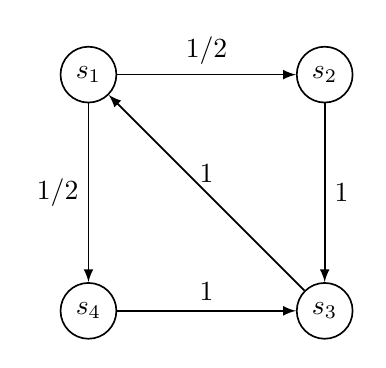
\begin{tikzpicture}[-latex ,auto , node distance =3 cm ,semithick,
        main/.style = {draw, circle}] 
            \node[main] (1) {$s_1$}; 
            \node[main] (2) [right of=1] {$s_2$};
            \node[main] (3) [below of=2] {$s_3$};
            \node[main] (4) [below of=1] {$s_4$};
            \draw (1) -- node[midway] {1/2} (2);
            \draw (1) -- node[midway,left] {1/2} (4);
            \draw (2) -- node[midway] {1} (3);
            \draw (3) -- node[midway,above] {1} (1);
            \draw (4) -- node[midway] {1} (3);
        \end{tikzpicture}
    \end{center}
Observando este grafo, podemos ver que todos los estados tienen periodo 3. Es más, todos los estados son comunicables entre ellas luego la cadena es irreducible. En definitiva, tenemos una cadena de Markov periódica con periodo 3.
\end{exampleth}

\subsection{Tiempos de transición}
Al inicio de esta sección habíamos visto las probabilidades de transición de $n$ pasos del estado $s_i$ al estado $s_j$. Con frecuencia queremos hacer afirmaciones en término de probabilidades sobre el número de transiciones necesarias para ir del estado $s_i$ al estado $s_j$, al que denominaremos \textit{tiempo de transición de $s_i$ hasta $s_j$}.\\

Cuando $s_i=s_j$, este tiempo es justo el número de transiciones que se necesita para regresar al estado inicial $s_i$. En este caso, este tiempo lo denominaremos \textit{tiempo de recurrencia para el estado $s_i$}.

\begin{definition}
Sea $\{\mathcal{X}_t\}$ una cadena de Markov. La variable aleatoria:
\begin{center}
    $\tau_{ij} := $ min$\{t\in\mathbb{N}\,|\, \mathcal{X}_t=s_j$ dado $\mathcal{X}_0=s_i\}$, considerando min $\emptyset$ = $\infty$
\end{center}
representa el tiempo mínimo que la cadena necesita para ir desde $s_i$ hasta $s_j$ y se conoce como \textbf{tiempo de transición de $s_i$ hasta $s_j$}. La variable $\tau_{ii}$ se llama \textbf{tiempo de recurrencia para el estado $s_i$}.
\end{definition}